\documentclass[tikz]{standalone}
\input{../tikz/plots_config.pgs}

\begin{document}

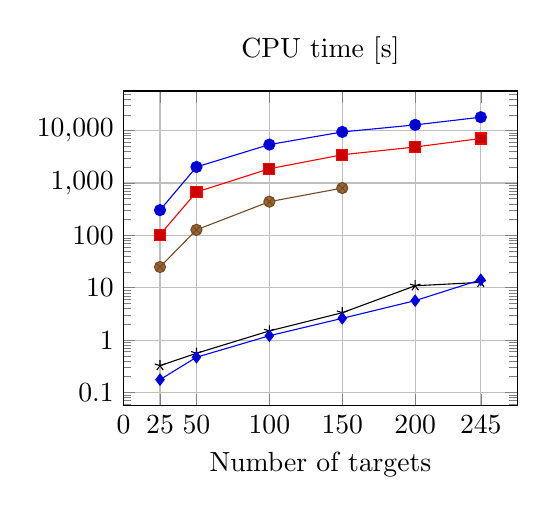
\begin{tikzpicture}
\begin{semilogyaxis}[%
log ticks with fixed point,
max space between ticks=20,
width=50mm,
height=40mm,
scale only axis,
xmin=0,
xmax=270,
xtick={ 0,  25,  50, 100, 150, 200, 245},
xmajorgrids,
ymajorgrids,
title={CPU time [s]},
xlabel={Number of targets},
]
% GLKH (iters=3000)
\addplot coordinates{
(25, 303.605389118)
(50, 2024.97808385)
(100, 5416.12343001)
(150, 9432.07198)
(200, 12862.167078)
(245, 18036.815737)
};

% GLKH (iters=1000)
\addplot coordinates{
(25, 103.231865168)
(50, 671.104985952)
(100, 1869.03779197)
(150, 3460.32806897)
(200, 4870.32181096)
(245, 7076.76331496)
};

% GLKH (iters=200)
\addplot coordinates{
(25, 24.9032230377)
(50, 127.74444294)
(100, 439.610677958)
(150, 800.083540916)
};

% TSP C-Space
\addplot coordinates{
(25, 0.325886964798)
(50, 0.561913013458)
(100, 1.50004410744)
(150, 3.3386118412)
(200, 10.9209008217)
(245, 12.6818139553)
};

% RoboTSP
\addplot coordinates{
(25, 0.176025867462)
(50, 0.471691131592)
(100, 1.21360182762)
(150, 2.60831999779)
(200, 5.67717385292)
(245, 14.213570118)
};
\end{semilogyaxis}
\end{tikzpicture}

\end{document}
